\def\homeworknumber{3}
\def\homeworkdate{24-10-2011}

\documentclass[11pt]{article}
\linespread{1}

\renewcommand{\thefootnote}{\fnsymbol{footnote}}

\usepackage{geometry} % see geometry.pdf on how to lay out the page. There's lots.
\usepackage[utf8]{inputenc}
\usepackage[T1]{fontenc}
\usepackage{array}
\usepackage{amsmath,amssymb,latexsym,epic,eepic,epsfig,graphics,psfrag}
\usepackage{amsfonts}
\usepackage{graphicx,float}
\usepackage{color}
\definecolor{mygray}{RGB}{244,244,244}
\definecolor{gray}{gray}{0.5}
\definecolor{myredish}{RGB}{193,33,97}
\definecolor{grayblue}{RGB}{91,112,142}
\definecolor{myorange}{RGB}{255,134,0}
\definecolor{green}{rgb}{0,0.4,0}

\usepackage[english]{babel}

\usepackage[bottom]{footmisc}

\usepackage{fancyhdr}
\pagestyle{fancy}
\lhead{\small\textit{Assignment \assignmentnumber -- 02417 Time Series Analysis -- Anders Hørsted (s082382)}}
\rhead{\thepage}
\chead{}
\lfoot{}\cfoot{}\rfoot{}

\usepackage{subfigure}
\usepackage{pstricks}
\usepackage{pst-node}
\usepackage{wrapfig}
\usepackage{caption}
\usepackage{multirow}
%\usepackage{fouriernc}
%\usepackage[charter]{mathdesign}
\usepackage{lmodern}
\usepackage[normalem]{ulem}
\geometry{a4paper} % or letter or a5paper or ... etc
% \geometry{landscape} % rotated page geometry

\usepackage{url}


\makeatletter
\renewcommand*\env@matrix[1][*\c@MaxMatrixCols c]{%
  \hskip -\arraycolsep
  \let\@ifnextchar\new@ifnextchar
  \array{#1}}
\makeatother

\newcommand\myimp{\quad\Leftrightarrow\quad}
\newcommand\half{\frac{1}{2}}
\newcommand\myvec[1]{\mathbf{#1}}
\newcommand\mymod[1]{\ (\text{mod }#1)}
\newcommand\myreal{\mathbb{R}}
\newcommand\mynatural{\mathbb{N}}
\newcommand\myinteger{\mathbb{Z}}
\newcommand\mycomplex{\mathbb{C}}
\newcommand\myint{\text{int}}
\newcommand\norm[1]{||\,#1\,||}
\newcommand\bignorm[1]{\big|\big|\,#1\,\big|\big|}
\newcommand\seq[1]{\big\{#1\big\}}
\newcommand\smallseq[1]{\{#1\}}
\newcommand\smallseqtoinf[1]{\smallseq{#1}_{k=1}^\infty}
\newcommand\lonew{\ell^1_w}
\newcommand\lone{\ell^1}
\newcommand\ltwo{\ell^2(\mynatural)}
\newcommand\ip[2]{\langle#1,#2\rangle}
\newcommand\hilbert[1]{\mathcal{#1}}
\newcommand\uinf{u_{\infty}}
\newcommand\erf{\text{erf\,}}
\newcommand\infint{\int_{\infty}^{\infty}}
\newcommand\fpi{FPI}
\newcommand\E[1]{\text{E}[#1]}
\newcommand\Var[1]{\text{Var}[#1]}
\newcommand\Cov[1]{\text{Cov}[#1]}
\newcommand\myverb[1]{{\footnotesize\texttt{#1}}}
\newcommand\Yhat{\widehat{Y}}
\newcommand\given{\,|\,}

\usepackage[scaled]{beramono}
\usepackage{listings}
\lstset {                 % A rudimentary config that shows off some features.
    language=R,
    basicstyle=\scriptsize\ttfamily, % Without beramono, we'd get cmtt, the teletype font.
    commentstyle=\textit, % cmtt doesn't do italics. It might do slanted text though.
    keywordstyle=,
    identifierstyle=,
    framextopmargin=4pt,
    framexbottommargin=4pt,
    framexleftmargin=4pt,
    framexrightmargin=4pt,
    xleftmargin=4pt,
    xrightmargin=4pt,
    backgroundcolor=\color{mygray},
    frame=single,
    showstringspaces=false,
    captionpos=b,
    tabsize=4            % Or whatever you use in your editor, I suppose.
}

\renewcommand{\lstlistlistingname}{Code Listings}
\renewcommand{\lstlistingname}{Code Listing}

\usepackage{tabulary}
\newcolumntype{y}{>{\centering\arraybackslash}R}

\title{\assignmenttitle}
\date{\assignmentdate}
\author{Assignment \assignmentnumber\ -- 02417 Time Series Analysis -- Anders Hørsted (s082382)}
%\author{}
\date{} % delete this line to display the current date



\begin{document}
    \maketitle

    \section*{Exercise 1}
    The annulus $A$ is given in polar coordinates by $r\in(1,2), \theta\in(0,2\pi)$. A PDE problem is defined by
    \begin{gather}
        \Delta u = 0 \text{ in }A \\
        u(1,\theta) = 0,\quad \frac{\partial u}{\partial r}(2,\theta) = 1 - 2\cos(\theta),\quad \theta\in(0,2\pi)
    \end{gather}
    The solution to this PDE problem is now found. The solution formula 6.4.7 in the textbook can be used for this problem. Using the first boundary condition we get that
    \begin{align*}
        u(1,\theta) &= \frac{1}{2}(C_0 + D_0\log(1)) + \sum_{n=1}^\infty (C_n+D_n)\cos(n\theta) + (A_n+B_n)\sin(n\theta) \\
        &\overset{\text{set}}{=} 0
    \end{align*}
    from which we conclude that $C_0=0, C_n=-D_n, A_n=-B_n$. Since
    \begin{align*}
        u_r(r, \theta) = \frac{1}{2}D_0r^{-1} + \sum_{n=1}^\infty (C_n n r^{n-1} - D_n n r^{-n-1})\cos(n\theta) + (A_n n r^{n-1} - B_n n r^{-n-1})\sin(n\theta)
    \end{align*}
    we get from the second boundary condition that
    \begin{align*}
        u_r(2, \theta) &= \frac{1}{4}D_0 + \sum_{n=1}^\infty (C_n n 2^{n-1} - D_n n 2^{-n-1})\cos(n\theta) + (A_n n 2^{n-1} - B_n n 2^{-n-1})\sin(n\theta) \\
        &= \frac{1}{4}D_0 + \sum_{n=1}^\infty (2^{n-1} + 2^{-n-1})C_n n \cos(n\theta) + (2^{n-1} + 2^{-n-1})A_n n \sin(n\theta) \\
        &\overset{\text{set}}{=} 1 - 2\cos(\theta)
    \end{align*}
    from which we get that $D_0=4, C_1=-\frac{8}{5}, D_1=\frac{8}{5}$ and all other coefficients should be 0. The solution is therefore given by
    \begin{equation*}
        u(r, \theta) = 2\log{(r)} + (\frac{8}{5}r^{-1} - \frac{8}{5}r)\cos(\theta)
    \end{equation*}
    The solution is plotted and is shown in figure~\ref{fig:q1-plot}. COMMENT!!
    \begin{figure}
        \centering
        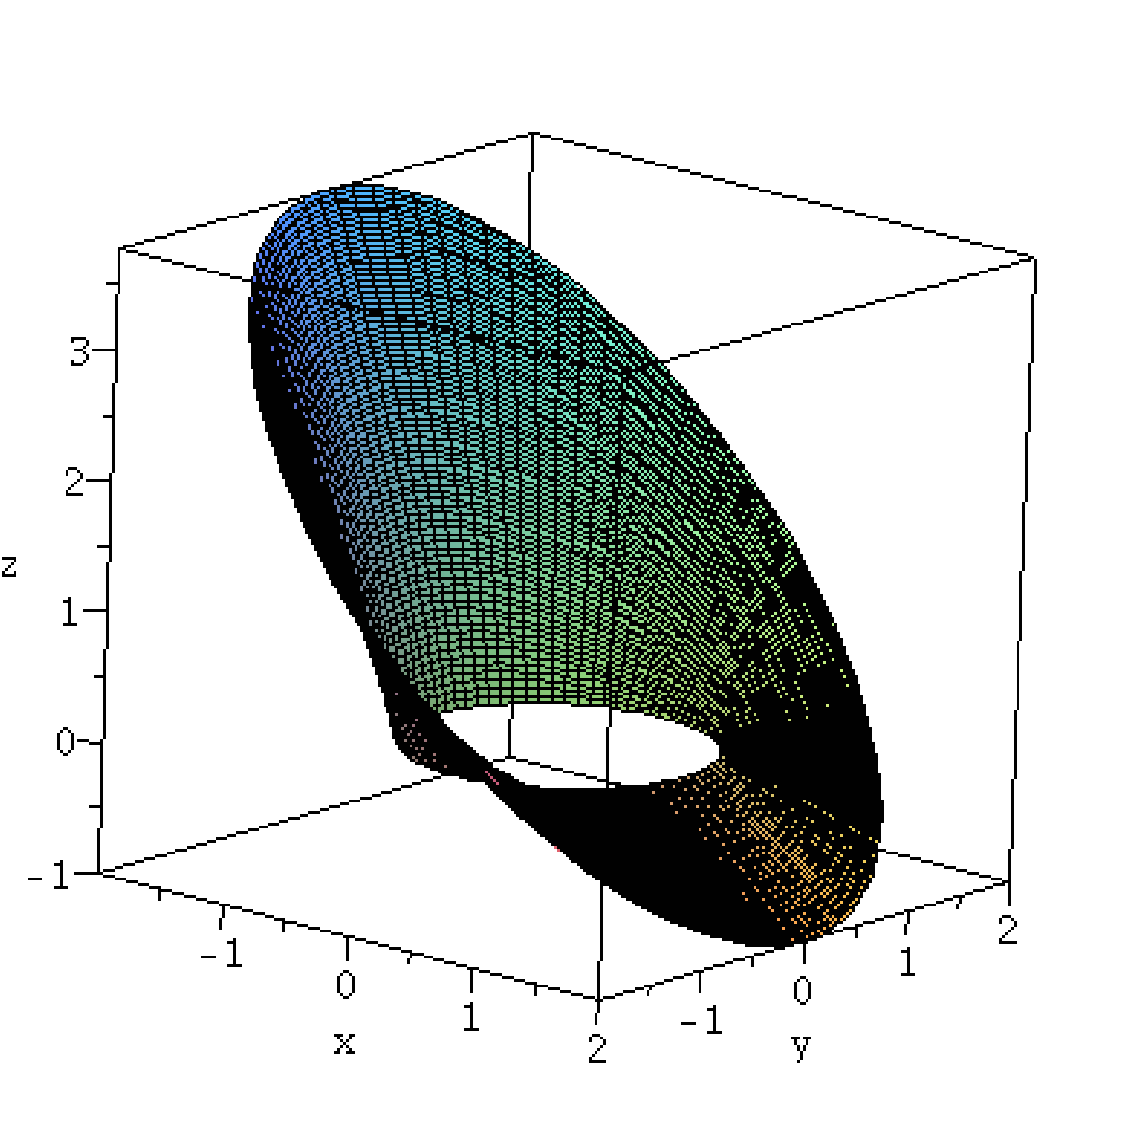
\includegraphics[width=80mm]{q1-plot.pdf}
        \caption{Plot of solution for exercise 1}
        \label{fig:q1-plot}
    \end{figure}

    \section*{Exercise 2}
    Using the reflection method the Green's function $G$ for the Laplace Equation in the half plane $H=\{(x,y)\,|\,x\in\myreal,\:y>0\}$ is found. Based on the derivation of the Green's function in the half space in the textbook combined with the representation formula in two dimensions (eq. 7.2.5) a good guess for $G$ is
    \begin{equation*}
        G(\vecx, \vecx_0) = \frac{1}{2\pi}(\log|\vecx-\vecx_0| - \log|\vecx-\vecx_0^*|)
    \end{equation*}
    that in coordinates becomes
    \begin{equation}\label{eq:green-coord}
        G(\vecx, \vecx_0) = \frac{1}{2\pi}(\log((x-x_0)^2 + (y-y_0)^2)^{1/2} - \log((x-x_0)^2 + (y+y_0)^2)^{1/2})
    \end{equation}
    By exactly the same arguments as in the textbook p. 191-192 it can be ``proved'' that $G$ is the Green's function for $D$ at $\vecx_0$. \par
    We now use $G$ to solve the Dirichlet problem
    \begin{gather*}
        \Delta u = 0 \text{ in } H, \\
        u(x, 0) = \begin{cases}
            1, & x\in(-1,1) \\
            0, & \text{elsewhere}
        \end{cases}
    \end{gather*}
\end{document}
